\documentclass{article}


\usepackage{graphicx} % Required for inserting images
\usepackage{biblatex} %Imports biblatex package
\usepackage{longtable}
\usepackage{rotating} % Required for sideways table



\addbibresource{references.bib} %Import the bibliography file


\title{Preprint submission}
\author{Christian Magelssen}
\date{February 2024}

\begin{document}

\maketitle

\section{Introduction}

The hallmark of expertise lies in the flawless execution of actions and the selection of optimal choices to achieve goals  \cite{wolpert_principles_2011, krakauer_motor_2019, mangalam_investigating_2023, du_relationship_2022, gallivan_decision-making_2018}. These choices (or cognitive strategies) are typically trained with instruction-based approaches, where a coach tells learners what to do (e.g., take a shorter line around the gate) followed by corrective feedback (e.g., you can shorten the line even more) \cite{williams_practice_2005, williams_effective_2023, hodges_role_1999}. This teaching strategy can be likened to what motor learning refers to as supervised learning, where the teaching signal for skill improvement represents the disparity between the desired skill outcome and the learner outcome \cite{jordan_forward_1992, wolpert_motor_2010, doya_complementary_2000}. Through practice this teaching signal can bring the learner closer to execute what is assumed to be the correct choice, but does this teaching approach truly foster creativity and intelligent strategic choices, such as helping learners discover innovative and vastly more effective solutions that surpass our imagination?

One drawback of the supervised learning strategy for training these decisions is that learners are simply told what to do based on what coaches believe to be a good strategy from their knowledge or experience. However, what coaches judge as a good strategy does not always align with reality, even for the best-trained eye \cite{supej_impact_2019, cochrum_visual_2021}. Learners might, therefore, miss opportunities to discover the best strategy when coaches opt for suboptimal choices \cite{gray_plateaus_2017}. Supervised learning might also constrain learners to adopting a single ('universal') strategy for all situations rather than acquiring a repertoire of strategies and discerning the most effective strategies for each specific scenario. Finally, it remains uncertain whether the prescriptive approach is the most effective teaching strategy for achieving long-lasting learning effects \cite{wulf_instructions_1997} 

Learning to make good choices can also happen without the direct influence of a coach who gives advice. The cornerstone of reinforcement learning \cite{sutton_reinforcement_2018} is that learners can learn by exploring strategies and evaluating their outcomes, using the successes and failures of outcomes as teaching signals. That is, rather than being told the putatively correct solution to the problem, as in supervised learning, they learn about the value of different strategies, which allows them to pick the best solution. These values are learned by comparing a given choice's outcomes with the currently expected outcome of that choice. Outcomes that exceed or fall short of expectations result in errors in reward prediction, signaling that the learner must update their predictions to better anticipate future rewards following that action \cite{rescorla_theory_1972}. These reward prediction errors are then incorporated to form a new and better estimate of reward, by updating expectations through a weighted running average. Reinforcement learning has been tremendously powerful in explaining human and animal learning \cite{waelti_dopamine_2001, schultz_neural_1997, pessiglione_dopamine-dependent_2006}, as well as training AI to perform complex tasks such as computer games starting from pixel inputs, only\cite{mnih_human-level_2015}. Given this evidence, could reinforcement learning offer an alternative to standard coach-based supervised learning to improve strategy selection and performance for skilled performers?

Advancing strategy choices in elite performers, however, extends beyond merely selecting an effective strategy; it entails consistently seeking new and better methods, a defining characteristic of deliberate practice \cite{ericsson_development_2003, ericsson_expert_1994, ericsson_role_1993}. Sometimes, achieving substantial performance improvements requires making radical shifts in strategy choices \cite{taylor_role_2012, gray_plateaus_2017}. Such switches require learners to enter a deliberate mode of action selection where they reorganize their mental representation of the skill to come up with even better strategies and performance\cite{du_relationship_2022}. How learners decide on, learn, and develop strategies is not currently known\cite{taylor_role_2012}, especially not in expert performers. Our question was whether reinforcement learning could contribute to better strategy selection than traditional supervised learning by allowing learners to experiment with strategies and evaluate their effects. 

To address this question, we conducted a three-day learning experiment with ninety-eight skilled and elite alpine ski racers from Norway and Sweden. To facilitate skill development in this skilled group of athletes, we selected a section of a slalom course where there is great improvement potential, even among the best skiers. This skill was to improve times on flat sections in slalom, and we defined four strategies intentionally to enhance this skill (\ref{fig:courseandstrategies}b). Our hypothesis was that skiers in the reinforcement learning group would learn to choose better strategies and thus achieve better performance than skiers subject to traditional supervised learning with a coach. To test this, we assigned skiers to three different learning groups with different instructions and feedback (Fig. \ref{fig:experiment}b): In the reinforcement learning group, skiers chose a strategy on every run and saw their race times to inform these decisions. In the supervised (free choice) learning group, a ski coach made this choice for the skier, while in the supervised (target skill) learning group, we recruited current World-Cup ski coaches to instruct skiers to select the strategy that we defined as the theoretically best strategy based on computational modeling \cite{lind_physics_2013} and observations of elite skiers \cite{reid_alpine_2020}. Coaches in the two supervised learning groups saw the times but were instructed not to disclose them to the skiers. 

We found that the reinforcement learning group showed greater improvement during acquisition and performed better in retention compared to the supervised (free choice) learning group. We observed an improvement in strategy choices for both reinforcement learning and supervised (free choice) learning groups, but we did not observe any statistically significant differences in choices between groups, either for the theoretically best strategy or individual skiers' estimated best strategy. We also found that both groups were sensitive to performance feedback, exhibiting win-stay, lose-shift behavior in strategy choices, but the descriptively greater sensitivity to feedback in the reinforcement learning group was not statistically significant. Our results suggest that reinforcement learning yields comparable outcomes to supervised learning, and that any advantages of reinforcement learning over supervised learning are more likely rooted in effects on skill execution rather than action selection. 



\begin{figure}[ht]
\centering
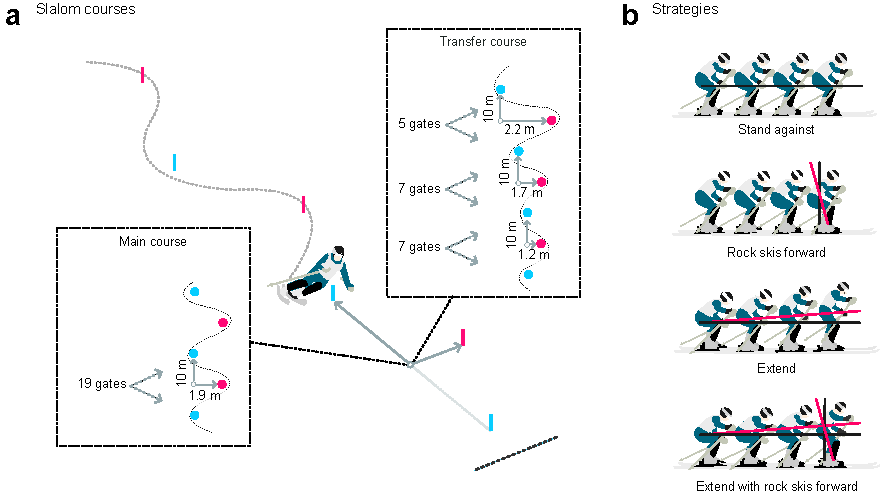
\includegraphics{figures/figure_method_courseandstrategy.pdf}
\caption{\textbf{a.} Illustrations of the two slalom courses used in the study. The main slalom course was a rhythmic course deployed in all sessions except for the transfer test. The course setting for the transfer test involved a progression in gate offset, starting with the largest offset and ending with the smallest offset. \textbf{b.} Illustration of the strategies defined to enhance racing performance on flat terrain in slalom: The "stand against" strategy emphasized maintaining a stable stance against external forces without body extension along the body's longitudinal axis or rocking skis forward; 'Rock skis forward' involved rocking skis forward from gate passage to completion of the turn; The "extend" strategy involves extending the body from a laterally tilted position during the turn, closer to the turn's center of rotation; The "extend with rocking skis forward" was expected to be the best strategy combining the two effects from extending and rocking skis forward, and we therefore defined this as the theoretical best strategy}
\label{fig:courseandstrategies}
\end{figure}

\begin{figure}[ht]
\centering
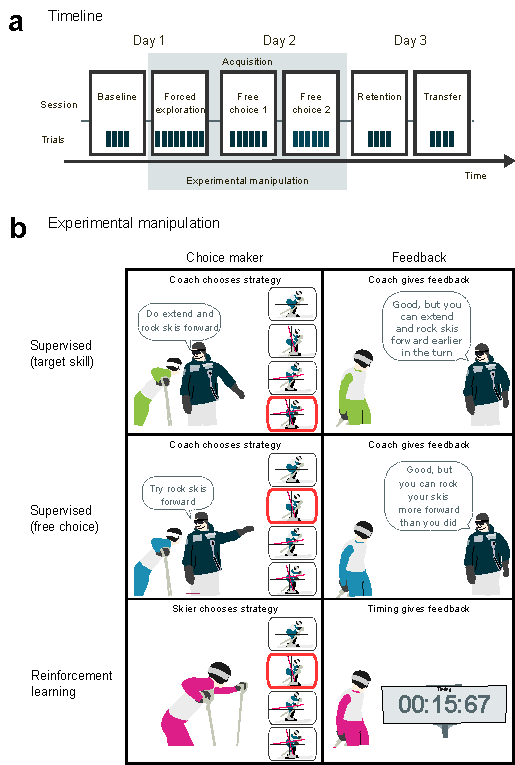
\includegraphics{figures/figure_method_experiment.pdf}
\caption{Illustration of the experimental design and procedure. \textbf{a.} Timeline of the three-day skill learning experiment. During the baseline, skiers skied a slalom course as fast as they could without receiving racing time feedback. The skiers' performances were ranked to form blocks. Within each block, skiers were randomly assigned to one of three treatment groups (see b).Skiers underwent an acquisition phase in their designated treatment group comprising one forced exploration and two free-choice sessions. On the last day, skiers completed a retention and transfer test, again without feedback from coaches nor timing. \textbf{b.} Illustration of treatment groups in the study. Supervised (target skill) involved coaches consistently choosing the theoretically best strategy, while supervised (free choice) allowed coaches to select strategies freely. Skiers in both these treatment groups received feedback on strategy execution from their respective coach, while skiers in the reinforcement learning group independently selected strategies and received feedback from the timing system to facilitate value learning of each strategy. }
\label{fig:experiment}
\end{figure}





\section{Discussion}

Expert performance relies on selecting and executing effective strategies with precision. The conventional method for training these decisions involves instructing learners on which strategy to choose. Our question was whether reinforcement learning could improve strategy selection and performance among adept alpine ski racers. Our findings indicate that reinforcement learning can complement traditional training methods and serve as a functional approach specifically tailored to train decision-making skills. We suggest that coaches can improve skill acquisition by crafting strategies and enabling learners to glean insights into their outcomes through evaluations rather than solely relying on direct instruction. 


\subsection{Race time}
Interestingly, the reinforcement learning group improved their race more during acquisition and had better retention than did the supervised (free-choice) learning group. This result accords first with prior studies on the 'discovery learning' approach, where practice without explicit instruction yields better learning effects \cite{wulf_instructions_1997, hodges_learning_2001}. More specifically, this finding aligns with earlier studies in reinforcement learning, which have demonstrated that learning through reinforcement feedback increases retention\cite{therrien_effective_2016, truong_error-based_2023, hasson_reinforcement_2015}. The presumed explanation behind these findings is that reinforcement enhances offline improvements in motor memories that are not observed with other learning paradigms. 

Although reinforcement learning also demonstrated descriptively better race times than supervised learning during the acquisition phase and retention, these differences were not significant. The strategy selected thus appeared to have been effective for this group. However, the advantage of using this strategy seemed to diminish over the course of the sessions, as this group experienced a descriptive decline from the first to the last free choice sessions in the acquisition phase. One possible explanation for this is that the strategy lost its effectiveness. We will discuss this more in..

Our hypothesis was also that reinforcement learning improves transfer to a new slalom course. The rationale for such expected behaviour was that reinforcement learning would achieve better insights into to the strategies' effect, thereby promoting better decision-making in new situations. However, we found no corroborating evidence for this hypothesis. This result aligns with studies that have observed enhanced retention but not transfer with reinforcement compared to supervised learning \cite{hasson_reinforcement_2015}. Furthermore, reinforcement learning has been found to yield a lower generalization signature in adaptive tasks \cite{lior_shmuelof_overcoming_2012}. One account for these findings is that reinforcement learning improves learning only for the specific situations in which one has been rewarded, as these are the instances in which learning has been reinforced. A potential mechanism for this is that training with rewards shortens the time window during which memory is unstable, affecting learners' capacity to extend learning to new situations \cite{robertson_memory_2018}. It is also conceivable that a more structured learning approach, where learners are exposed to frequent switches between strategies, is necessary to grasp the task's structure and promote transfer \cite{braun_structure_2010}. Future research should possibly investigate the effect of structural learning. 

\subsection{Choices and learning}
Our initial explanation for the improved acquisition and retention in the reinforcement learning group was that they learned to choose better strategies through evaluation via choice. During acquisition, we found that reinforcement learning enhanced its choices, while we did not observe the same evidence for supervised (free choice) learning. Both groups exhibited a 'win-stay, lose-switch' signature, indicating a tendency to stick to successful strategies. Despite reinforcement learning showing a descriptive tendency to select better strategies and having more pronounced "win-stay, lose-switch" tendencies during acquisition, these differences were not statistically significant, contrary to our initial hypothesis. 

Similar 'win-stay, lose-switch' tendencies have been found in other motor learning studies. The finding of 'win-stay, lose-switch' in our study suggests that elite sportspeople seek effective strategies. One plausible explanation for not finding corroborating evidence for group differences in choice or on 'win-stay, lose-switch' is that we were dealing with highly experienced coaches with solid sports knowledge. Therefore, we should be cautious in describing this as a null result. It is also important to note that coaches had access to skiers' race times and underwent significant learning too. In a typical training situation, coaches might not have tested strategies as extensively as in this study.  

A surprising finding was that supervised (free choice) learning had a descriptively higher predicted probability of choosing the skier's estimated best strategy on retention. Still, the reinforcement learning had the fastest race times during retention. One interpretation of this result is that skiers in the reinforcement learning group took into consideration the variability of performing a strategy and opted for those with lower incurred risk, despite another strategy being more effective. This understanding may have arisen because skiers in the reinforcement learning group discovered that multiple strategies led to similar outcomes and chose the slightly worse strategy due to lower variability. In that case, one might consider that "extend with rock skis forward" to be more risky since it could potentially make athletes lean too far backward to be able to engage the skis in the next turn. However, this does not seem to be a good account of our data as the choices of this strategy increased on retention. A more likely explanation is that that the skiers in reinforcement learning built a better mental representation of the strategies and learned that two or more produced the same outcomes, and just picked any of them.

This explanation, however, cannot fully account for the disparity in race time. Compared with supervised (free choice) learning, reinforcement learning achieved greater improvement in the 'extend' strategy, suggesting that reinforcement feedback might have increasing motor vigor \cite{pietro_mazzoni_why_2007, dudman_basal_2016}, such that their "energized" this action better. Indeed, previous studies have found that people make saccades \cite{takikawa_modulation_2002} and reach\cite{summerside_vigor_2018} faster towards targets paired with rewards than unpaired targets. Comments from a few coaches, who watched the retention and transfer, from the sideline, uttered that skiers in the reinforcement learning group used more forceful arm movements than skiers in the other groups, despite the instruction did not tell them to do that.

The vigor perspective may also help explaining why reinforcement learning did not learn better than the supervised (target skill) learning group, as previous studies also have found that training with explicit knowledge boosts motor vigor much like the effect of reward itself \cite{anderson_rewards_2020, wong_explicit_2015}. It may therefore be that the getting information from a current World Cup coach that one strategy was best boosted the implicit motivation to perform this strategy well. 


Our study suggests that reinforcement learning can be an essential training strategy to improve skill acquisition. However, before encouraging coaches and instructors to implement this strategy, we discuss the significance of the effect size and its amplifying and counteracting mechanisms for generalizability \cite{anvari_not_2023}. To start this discussion, we emphasize that the estimated effect size during retention was smaller than our predefined smallest effect size of interest. This benchmark, however, was set for a longer slalom course and more training sessions than we could execute due to space and time constraints in the ski hall. Consequently, we exercise caution in outright dismissing its practical significance. Instead, we aim to help the reader understand its potential importance for skill improvement in our sample of skiers. The first step towards this insight is to consider that the slalom course approximately equaled one-third of a full slalom race course, and a slalom race consists of two runs. Therefore, the 0.12 seconds effect size could be scaled up by a factor of 6, potentially proving significant for coaches in a more accurate course setup. However, racecourses consisting solely of flat sections are rare, and it is more realistic to assume that a flat section of a course constitutes only one-third of the entire course. If we base our understanding on this assumption, we can convert the 0.12-second difference into FIS world ranking positions. Considering that a race consists of two runs, this translates into an improved World Rank of 27 positions for females and 65 for males, based on a median ranking of 600 in our sample (see Supplement discussion). This could be of significant importance, but we have to remember that this effect cannot be directly transferred, as sports expertise also involves cognitive decisions \cite{mangalam_investigating_2023, krakauer_motor_2019}, such as switching from one strategy to another during a race. Our study did not capture such decisions as we focused on flat sections. In conclusion, the estimated effect could be larger if not because reinforcement learning and supervised learning conducted the retention and transfer tests simultaneously. This design choice allowed the skiers to observe each other, possibly diluting some of the effect. However, this decision was made to mirror the conditions of alpine competitions and gave us confidence that athletes experienced similar conditions during testing. 

\section{Methods}

\subsection{Participants}
We recruited ten alpine ski teams from Norway and Sweden comprising 98 alpine ski racers (age M = 18.1 years, SD= 2; 40 females, 58 males). Two skiers were excluded from the analysis due to an injury prior to the study (n=1) or sickness during the study (n=1); thus, a total of 96 skiers completed the entire study and were included in the analysis. We deliberately opted to recruit skiers with diverse skill levels for the study to augment the generalizability of our findings. However, to ensure a sufficient skill level to handle the specific icy snow conditions prepared in the skiing hall, we recruited only skiers aged 15 and older. Among the ski groups tested were five ski academies, three senior development teams, and two national ski teams. These skiers were generally highly skilled, with a median world rank of 605, but there was also considerable variability, as indicated by a substantial interquartile range (Q1 = 248, Q3 = 1390.5). A smaller subset of the participants (n = 13) was not world-ranked, as they had yet to record FIS points. Table 1 provides demographic information for each treatment group.

Conducting studies on alpine ski racing poses challenges related to environmental control and resource constraints. Our sample size approach involved recruiting as many skiers as possible during the summer of 2023, with a set minimum sample size of 80 skiers, which we deemed appropriate for this context. Prior to data collection, data and power simulations for sample sizes of 80, 100, and 120 skiers were conducted, revealing simulated powers of 0.60, 0.75, and 0.80, respectively, for the smallest effect size of interest (0.3 second difference between groups) (\url{https://osf.io/c4t28}). The smallest effect size of interest was based on our knowledge of alpine skiing and discussions with coaches, but it was intended for a 50-meter longer course and more training sessions than we ultimately ended up using due to practical considerations. The sample size justification, task design, and analysis plan were preregistered before data collection (\url{https://osf.io/tfb2w}).

Due to space and time constraints in the ski hall, it was not possible to test all the ski teams simultaneously. The 10 ski teams were therefore divided into 4 groups for which the study was conducted at different times. For each group that participated in the study, we recruited two coaches from the ski teams to serve as coaches in the supervised (free choice) learning group, totaling 8 coaches (2 women; 6 men). These coaches had extensive coaching experience in coaching alpine ski racers. In addition, for each group of ski teams that completed the experiment together, we recruited a third coach to coach the skiers in supervised (target skill) learning. To ensure that these coaches had sufficient credibility to make the skiers buy into our theoretical best strategy, we selectively recruited three highly experienced coaches from the Norwegian alpine ski team, with one coach serving twice due to illness of the fourth coach. Importantly, all the coaches remained unaware of the experimental manipulation. Table 2 provides demographic information of the coaches. All the skiers and coaches provided informed consent before the study. The study was approved by the Human Research Ethics Committee of The Norwegian School of Sport Sciences.



\begin{sidewaystable}
\caption{\textbf{Skier characteristics}}
\centering
\begin{tabular}[t]{l|c|c|c|c|c|c}
\hline
\multicolumn{1}{c|}{ } & \multicolumn{2}{c|}{\textbf{Reinforcement learning}} & \multicolumn{2}{c|}{\textbf{Supervised (free choice)}} & \multicolumn{2}{c}{\textbf{Supervised (target skill)}} \\
\textbf{Sex} & \textbf{F}, N = 13 & \textbf{M}, N = 19 & \textbf{F}, N = 14 & \textbf{M}, N = 19 & \textbf{F}, N = 13 & \textbf{M}, N = 20\\
\hline
Age & 18.4 (2.3) & 17.7 (1.8) & 18.1 (2.3) & 18.3 (1.8) & 17.8 (2.4) & 18.2 (2.1)\\
\hline
Training group &  &  &  &  &  & \\
\hline
\hspace{1em}National team & 1 (7.7\%) & 1 (5.3\%) & 2 (14\%) & 1 (5.3\%) & 2 (15\%) & 4 (20\%)\\
\hline
\hspace{1em}Senior team & 3 (23\%) & 5 (26\%) & 1 (7.1\%) & 5 (26\%) & 0 (0\%) & 5 (25\%)\\
\hline
\hspace{1em}Ski academy & 9 (69\%) & 13 (68\%) & 11 (79\%) & 13 (68\%) & 11 (85\%) & 11 (55\%)\\
\hline
FIS points &  &  &  &  &  & \\
\hline
\hspace{1em}Median (IQR) & 54 (42, 80) & 46 (34, 90) & 58 (26, 80) & 44 (35, 61) & 49 (28, 66) & 31 (28, 63)\\
\hline
\hspace{1em}Not recorded & 3 & 2 & 1 & 2 & 2 & \vphantom{1} 3\\
\hline
World ranking &  &  &  &  &  & \\
\hline
\hspace{1em}Median (IQR) & 630 (394, 1,217) & 707 (364, 2,317) & 709 (133, 1,224) & 662 (387, 1,274) & 527 (145, 882) & 314 (220, 1,360)\\
\hline
\hspace{1em}Not recorded & 3 & 2 & 1 & 2 & 2 & 3\\
\hline
\multicolumn{7}{l}{\rule{0pt}{1em}\textsuperscript{1} Mean (SD); n (\%)}\\
\end{tabular}
\end{sidewaystable}


\begin{sidewaystable}
\caption{\textbf{Coach characteristics}}
\centering
\begin{tabular}[t]{l|c|c|c}
\hline
\multicolumn{1}{c|}{ } & \multicolumn{2}{c|}{\textbf{Supervised (free choice)}} & \multicolumn{1}{c}{\textbf{Supervised (target skill)}} \\
\textbf{Characteristic} & \textbf{F}, N = 2 & \textbf{M}, N = 6 & \textbf{M}, N = 3\\
\hline
Age & 38.5 (3.5) & 44.3 (8.8) & 48.0 (7.0)\\
\hline
Ski education (highest achieved) &  &  & \\
\hline
\hspace{1em}Level 2 & 0 (0\%) & 1 (17\%) & \\
\hline
\hspace{1em}Level 3/4 & 2 (100\%) & 5 (83\%) & 3 (100\%)\\
\hline
Sport science degree (highest achieved) &  &  & \\
\hline
\hspace{1em}MSc & 1 (50\%) & 0 (0\%) & 1 (33\%)\\
\hline
\hspace{1em}BSc & 1 (50\%) & 1 (17\%) & 1 (33\%)\\
\hline
\hspace{1em}No & 0 (0\%) & 4 (67\%) & \\
\hline
\hspace{1em}One-year program & 0 (0\%) & 1 (17\%) & 1 (33\%)\\
\hline
Coaching experience (years) &  &  & \\
\hline
\hspace{1em}National team (WC/EC)/Senior teams & 5.00 (1.41) & 5.00 (4.24) & 15.67 (1.15)\\
\hline
\hspace{1em}Ski academy & 7.5 (3.5) & 7.5 (6.5) & 2.00 (3.46)\\
\hline
\hspace{1em}Ski club & 2.5 (3.5) & 6.5 (8.7) & 6.0 (6.6)\\
\hline
\multicolumn{4}{l}{\rule{0pt}{1em}\textsuperscript{1} Mean (SD); n (\%)}\\
\end{tabular}
\end{sidewaystable} 


\subsection{The setup}
The experiment was conducted in the indoor ski hall SNØ in Oslo, Norway (\url{https://snooslo.no/}). In this hall, we used a 210-meter-long flat section of the race hill, which we water-injected before testing each group of skiers to ensure uniform and fair snow conditions for all participants. For additional preparation details and images, please refer to Supplementary A. With our chosen course setup, this 210-meter-long flat section allowed space for 19 slalom gates. We sat two types of slalom courses in the experiment (Figure \ref{fig:design}a). The main slalom course was used in all sessions, except during the transfer test, and featured a 10 m distance and a 1.9 m offset. The course distance aligned with our previous study \cite{magelssen_is_2022}, but we opted for a slightly larger offset to better suit the skill level of our skiers. The transfer test aimed to evaluate how skiers transferred their learning to a slalom course that resembled a typical alpine ski racing course. To assess this, we set a course with a progression in gate offset, starting with five gates set at a 2.2-meter offset, followed by seven gates at a 1.7-meter offset, and concluding with seven gates at a 1.2-meter offset. Although we did not expect radical differences in strategy effects, we anticipated a greater emphasis on rocking the skis forward in gates with a 2.2-meter offset than in those with a 1.2-meter offset to enhance turn exit release. Both courses were set with stubbies (short gates) instead of long gates to minimize energy dissipation upon hitting the gate \cite{minetti_biomechanics_2018} and provide the skiers with space and freedom to execute the strategies. In addition, this approach helped us avoid creating holes in the course, which can occur when the long gate is forcefully slammed into the ground.

 The start gate was positioned 20 meters before the first gate. Skiers were required to start in a static position to ensure consistency in the starts, with their binding front head placed behind the starting gate. The skiers started by putting their skis in parallel and lifting up the poles without using poling or skating for propulsion. For an illustration of the starting procedure and setup, see Supplement Video. We recorded the times using a wireless photocell timing system (HC Timing wiNode and wiTimer; Oslo, Norway). Timing started when the skier crossed the first photocell pair situated 10 meters below the starting gate. To minimize wear and tear on the course, we set two parallel and identical courses and routinely shifted between them.
 
\subsection{Experimental design}
We employed a between-subjects design and posed the learning question of discovering effective strategies as an \textit{n}-armed bandit problem \cite{sutton_reinforcement_2018}. The essence of this problem is that a learner repeatedly tries different options and observes their outcomes to learn which strategy is the best and, therefore, which one to choose. Finding the best strategy requires a delicate balance between exploiting the strategy known to yield the best payoff and exploring alternative strategies that may offer superior benefits. In our study, the options consisted of four strategies that skiers could employ to improve their race times on flat slopes in slalom, grounded in physics-based coaching manuals for alpine ski racing \cite{lemaster_skiers_1999, lemaster_ultimate_2010, lind_physics_2013}, biomechanical research on elite skiers \cite{reid_kinematic_2010, tjorhom_beskrivelse_2007, reid_alpine_2020, magelssen_is_2022}  or common strategy used by coaches. The four strategies were named "stand against", "rock skis forward", "extend", and "extend with rock skis forward". (Figure 1\ref{fig:courseandstrategies}b for a strategy illustration and \ref{sup_strategies} for an extended explanation)

To study how instruction and feedback drive learning of strategy selection, we designed and allocated skiers to three treatment groups that allowed us to compared reinforcement learning with traditional supervised learning with a coach:

For the supervised (target skill) learning group, we provided the best possible training program by engaging highly experienced and meritorious coaches who explained to the skiers that the 'extend with rock skis forward' strategy was the most effective for skiing fast on flat terrain in slalom. They imparted this information, citing a previous doctoral project \cite{reid_kinematic_2010}, which revealed that the fastest slalom racers spent more time aft of the skis, emphasizing the involvement of a dynamic rocking movement. In addition, the coaches informed them that simulations of ski racers had yielded similar results \cite{mote_accelerations_1983, lind_physics_2013}. The coach then guided the skiers to adopt this strategy and provided feedback on its execution after each trial. Note that the coach had access to the skiers' times after each trial but were prohibited from sharing this information with the skiers.

In the supervised (free choice) learning group, skiers were assigned to two coaches recruited from the tested ski group. We recruited two coaches to minimize waiting time and thus enhance training efficiency. To balance the skiers' skill levels within the treatment group, we created new blocks from the ranked list from baseline testing and randomly assigned them to the coaches. We instructed the coaches to improve the skiers' racing times as much as possible using all four defined skiing strategies. During each trial, the coach would select a strategy for the skier, observe the skier during his trial and provide feedback on its execution afterward. Similar to the supervised (target skill) learning group, the coaches had access to the skiers' times after each trial but could not share this information with the skiers.

In contrast, the reinforcement learning group was not assigned any coach. Instead of having a coach deciding the skiing strategy for them, the skiers in this treatment group were told to choose a strategy for each trial by themselves to ski the course as fast as possible. To help the skiers choose and learn from their choice and skiing execution, this group could see their racing times immediately after they crossed the finish line. Although this group had no coach, we assigned a person to communicate with the skiers to record their choices and encourage them to try skiing fast, also to equalize out some of the motivational effect of having a coach in the other treatment groups. 

\subsection{Procedures}\label{subsec4}
Figure \ref{fig:experiment}a illustrates the procedures employed in the study. 
In the baseline test, skiers began with two warm-up runs: one in free skiing warm-up course and one specific warm-up in the slalom course. During these warm-up runs, skiers were instructed, trained and verified on the start procedure and start technique by an instructor. As a first run in the baseline assessment, skiers completed a straight-gliding run, where they skied straight down from start to finish in a static, upright slalom posture. Subsequently, the skiers completed four runs in the slalom course. Skiers were encouraged to ski as quickly as they could, but they could not see their times, nor did they get any instruction on how to perform well. 

After the initial baseline assessment, the skiers took a 60-minute break. In the meantime, we allocated the skiers to the three treatment groups: reinforcement learning, supervised learning (target skill), and supervised learning (free choice). To allocate the skiers to groups, we deployed a randomized-blocked approach to account for pre-existing differences in the skiers’ performance levels \cite{maxwell_designing_2017}. Specifically, we computed each skier’s average performance across the four trials in the baseline and ranked them accordingly. We then created \textit{n} blocks with block sizes corresponding to our three treatments for the entire list of skiers and assigned these skiers to these predefined blocks. Finally, we randomly allocated the skiers to the different treatment groups within each block (Figure \ref{fig:experiment}b).

The treatment groups participated in sessions at different times to prevent treatment diffusion \cite{maxwell_designing_2017}. As the ski group comprised teams of skiers who know each other well and were residing together, we explicitly emphasized the importance of keeping information about the sessions private. To stay within the time frame at the ski hall, the two supervised learning groups underwent training together. To facilitate this, we arranged stations in the finish area with space and vision dividers and ample space to impede communication between coaches in the supervised learning groups. In addition, we developed a Python script that fetched racing times from the timing system, filtered the times for each coach, and transmitted it to the station where the coach was located, ensuring no information flow between coaches. The treatment group that initiated after the baseline session was randomized and counterbalanced across the group of ski teams we tested.

The first session after the treatment assignment involved a forced exploration. Here, skiers within the treatment group were gathered, and the session started by introducing them to the strategies. We explained that we had identified four strategies to enhance racing times on flats in slalom. Subsequently, each strategy was detailed, supported by illustrative drawings in \ref{fig:courseandstrategies}b Figure and corresponding word explanations as outlined in the \ref{subsec4}. To confirm comprehension, we conducted two short familiarization trials for each strategy, or until the execution met our performance standards. After reviewing the strategies with the participants, we gathered them in their respective treatment groups and asked them to rank the strategies online for what they believe are most to least suitable to improve performance in flat terrain slalom skiing. Throughout the instruction and ranking process, skiers were explicitly instructed not to discuss the strategies with each other. It is important to note that the same instructor was used for all treatment groups within a tested ski group. After this, the skiers conducted a total of eight trials on the course, with two trials for each strategy. During these trials, the reinforcement learning group got feedback from the timing whereas the coach gave feedback in the supervised learning. After completing the eight rounds, the skiers re-evaluated and ranked the strategies.

On the second day, skiers completed two free-choice sessions, each comprising a total of 6 trials in the same slalom courses that were used the baseline testing the day before. Prior to the 6 free - choice trials, the skiers performed one warm-up free skiing run and one warm-up run in the slalom course. In these sessions, supervised (target skill) learning consistently selected the theoretically best skiing strategy. Conversely, in supervised (free choice) and reinforcement learning, the coach and the skiers, respectively, had the autonomy to choose skiing strategy for each run. After each session, coaches (except supervised target skill) and skiers were asked to re-evaluate and rank the strategies.

On the third and last day, the skiers performed a retention and a transfer test to assess the effect of the training approaches on learning and performance. The retention test was performed in the same course as the baseline and acquisition sessions, whereas the transfer test was performed in the transfer course and involved a progression in gate offset from start to finish. Since the transfer test was a new course, we allowed the skiers to inspect the course before the test. The retention and transfer tests were conducted with all treatment groups together. None of the treatment groups received any feedback from coaches nor time during these tests. After each test, the skiers were asked to rank the strategies. 

\subsection{Analysis}

After the data were collected, the chosen strategies of skiers or coaches were manually inputted into the database. The resulting dataset, which included raw racing times and strategy choices, was downloaded as separate CSV files and stored in the 'data' folder. These files were subsequently imported into R (v4.2.2, 2022) and processed using custom functions built upon the base R and tidyverse packages . Information logged during the experiment, such as when skiers did not complete the course ('Did Not Finish'), was then added to the relevant trials in the dataset. After this, the data underwent a cleaning process, during which trials with implausible high or low racing times were detected and replaced with “not assessed” (NA). Instances where the timing system failed to start were manually added as trials with NA values, along with corresponding strategy information. Finally, the data underwent extensive validation, including trial counting and visual inspection of the racing times for errors. The validated dataset was saved as a new CSV file. An extensive report can be found at OSF (link when it is uploaded).

Due to the hierarchical structure of the data, our general statistical strategy relies on multilevel modeling. At the first level, each skier performed multiple trials during each session. At the second level, each skier was nested within groups of ski teams that performed the experiment together. To account for these multilevel data structures, we leveraged linear mixed-effects models. To model random effects, we adopted a design-driven approach \textbackslash{}cite\{barr\_random\_2013, barr\_learning\_2021\}, where we sought to account for all nonindependence introduced by repeated sampling from the same ski group and skier. We deployed classical frequentist statistics and fitted these models with the lme4 package \textbackslash{}cite\{bates\_fitting\_2015\} in the R programming language. Two-tailed p values and degrees of freedom for each model were derived using the lmerTest package \textbackslash{}cite\{kuznetsova\_lmertest\_2017\} via the Satterthwaite approximation method. Alpha was set to 0.05 for all test statistics.

 \textbackslash{}subsubsection\{Racing time\}\label\{subsubsec4\}

Racing time was analyzed using linear mixed-effect regression models. Initially, we planned to normalize the racing time by expressing the racing time as the difference from the straight-gliding time performed at the beginning of every session. This difference better approximated the skiers' actual skill improvement by considering the variance in snow conditions. However, practical considerations led us to deviate from this approach. This change was due to either flipping or shifting of the course each day to ensure snow conditions with the least damage. Unfortunately, these adjustments made maintaining a clean, straight-gliding lane difficult since the straight gliding lane crossed many areas with damage to the snow surface (holes) from the previous course set. Collisions with these holes affected the number of racings, adding noise to the results. Therefore, we used a more conservative approach and analyzed the raw racing times instead of analyzing the normalized racing times.

 For the acquisition session, we modeled racing times using session (forced exploration, free choice 2, free choice 3) and treatment (reinforcement learning, supervised learning (free choice), supervised learning (target skill)) and their interactions as predictors. For retention and transfer, we modeled racing times at these sessions, with treatment added as a predictor. In addition, we used the average performance for each skier on the baseline test as a predictor to improve estimate precision and adjust for group differences at baseline testing. We used a simple coding scheme for our predictors where the intercepts represent the estimated mean of the cell means and the contrasts represent the estimated difference with respect to the reference level, which we set for reinforcement learning.

   \textbackslash{}subsubsection\{Strategy choices\}\label\{subsubsec4\}

 Skiing strategy choices were analyzed using generalized linear mixed-effect regression models with a binomial logit-link function.

 To model the selection of the theoretical best strategy, we inputted the data as logistic, where for each trial (\textbackslash{}(i\textbackslash{})) per skier (\textbackslash{}(j\textbackslash{})) within the ski group (\textbackslash{}(k\textbackslash{})), we counted \textbackslash{}(y\_{ijk\}=1\textbackslash{}) when the skier chose the theoretical best strategy (that is, 'extend with rock skis forward') or 0 when they did not. We included treatment and session and their interaction as two variables. To account for the nonindependence of the data structure, we allowed the intercept to vary by including a random intercept for the skier and ski groups.

 We adopted the same model formula to model the selection of the estimated best strategy. This time, however, we counted \textbackslash{}(y\_{ijk\}=1\textbackslash{}) when the skier chose their estimated best strategy or 0 when they did not select that strategy. To estimate the best strategy for each skier in the sample, we used the sample-average method \textbackslash{}cite\{sutton\_reinforcement\_2018\} to average the racing time for each strategy and select one of the strategies with the lowest estimated (that is, best) value. The following were used for the acquisition sessions: forced exploration, free choice 1, and free choice 2. Due to the scaling issues with generalized linear models, we followed the recommendation to determine the size and significance of the effects of interest using marginal effects on the probability scale \textbackslash{}cite\{mize\_best\_2019, mccabe\_interpreting\_2022\}. Interactions were assessed using discrete difference (also second difference), which is also in line with these recommendations. To derive these estimates, we used the emmeans package \textbackslash{}cite\{lenth\_emmeans\_2023\}.

 \textbackslash{}subsubsection\{Error sensitivity\}\label\{subsubsec4\}

 To learn how skiers and coaches used their feedback to guide their choices, we constructed a win-stay/lose-shift model (WSLS). For this WSLS analysis, we z scored the race times for each skier for free choices 1 and 2 and counted \textbackslash{}(y\_{ijk\}=1\textbackslash{}) when the skier repeated the previous strategy and 0 when it was not. The data were modeled using a generalized linear mixed-effect regression model with a binomial logit-link function, with treatment and race time (z-transformed) and their interaction as the two variables. To test for differences in error sensitivity, we used the marginal effects at the mean (MEM) derived from the emmeans package \textbackslash{}cite\{lenth\_emmeans\_2023\}.

 








nowak_strategy_1993


 
\section{Supplementary}




\subsection{Description of strategies}\label{sup_strategies}
This supplementary describes each strategy in more detail. 

The "stand against" strategy emphasized maintaining a stable stance against external forces without body extension along the body's longitudinal axis or rocking skis forward. This term is frequently used by Norwegian ski coaches when communicating with skiers to help them improve their race times. 

The "rock skis forward" strategy involves rocking the ski forward during the turning phase. This action effectively regulates the distribution of pressure over the skis. During the initiation and control phases of a turn, the pressure is generally shifted forward to bend the ski's forebody, increasing friction with the snow and enabling it to turn more sharply. However, at some point, during turn progression, the skier aims to stop turning and therefore shifts the pressure further back on the skis, thereby reducing turning and braking forces \cite{lemaster_skiers_1999, lemaster_ultimate_2010}. Investigations of elite alpine ski racers have shown that high performing skiers tend to rock skis more forward and pressure the back part of the ski for considerable longer time during a turn, than slower skiers \cite{reid_kinematic_2010, tjorhom_beskrivelse_2007, reid_alpine_2020}. To make the information more specific for the skiers, we communicated, that the maximum range of the rocking movement was about 30-50 centimeters from gate passage to completion of the turn, which is in correspondence with biomechanical evidence of elite ski racers \cite{reid_kinematic_2010}. 

The "extend" strategy involves extending the body from a laterally tilted position during the turn, closer to the turn's center of rotation. This pushing motion leads to more proper handling of a reservoir of energy available when skiers lower their bodies in the switch between turns. When skiers extend their bodies, while being laterally inclined in the slalom turn, they create ground reaction force. The radial component of the ground reaction force moving the center of mass closer to the center of rotation increases velocity, in accord with the principle of mechanical energy conservation \cite{lind_physics_2013}. Simulation studies of individuals extending their body in rollers or during carved slalom turns have shown that this movement can increase speed \cite{mote_accelerations_1983,luginbuhl_identification_2023}, and the effect has been observed in various ways with elite skiers during training and competition \cite{reid_kinematic_2010, magelssen_is_2022, supej_differential_2008}. 

Finally, "extend with rocking skis forward" was expected to be the best strategy combining the two effects from extending and rocking skis forward, and we therefore defined this as the theoretical best strategy. Simulations of skiers extending their bodies in the bottom of a roller have observed an additional effect of rocking the skis forward \cite{mote_accelerations_1983}



\subsection{Snow preparation}\label{sup_snowprep}
We dedicated a substantial amount of time and effort to prepare the hill for our learning experiment. Our primary objective was to ensure that the snow conditions were as identical and fair as possible for all participants. To achieve this, we collaborated closely with the SNØ facility’s staff and the coaches of the Norwegian Alpine Ski team. Together, we devised a comprehensive plan to achieve consistency before each group of skiers took to the slopes. This report will detail the steps we took to ensure the snow was ready for our skiers and provide insight into the reasoning behind our choices. The purpose of this supplementary note is to assist you in evaluating our study and to transparently document our commitment to delivering the best possible conditions for our skiers.

\subsubsection*{Ski group A}
About two weeks before testing Group A, new snow was created on the racing hill. The evening before data collection, machines groomed the racing hill (Fig. \ref{fig:snowprep}a:left). We then watered the hill and left it to freeze overnight to create a hard and firm surface (Fig. \ref{fig:snowprep}a:right). 

\subsubsection*{Ski group B}
Ski group B began testing the day after ski group A completed their testing. Once group A finished, we inspected the race hill(Fig. \ref{fig:snowprep}b:left), noticed some small holes, and decided to fill them before watering it again (Fig. \ref{fig:snowprep}b:right).  

\subsubsection*{Ski group C}
After ski group B, the race hill started getting icy, lacking grip in some areas. We were concerned that watering it again might worsen conditions, making it too challenging for skiers. Consequently, we opted to gently groom the hill with a machine and let the grooves set for a couple of days. See figure \ref{fig:snowprep}c for the result of this process.

\begin{figure}[h!]
\centering
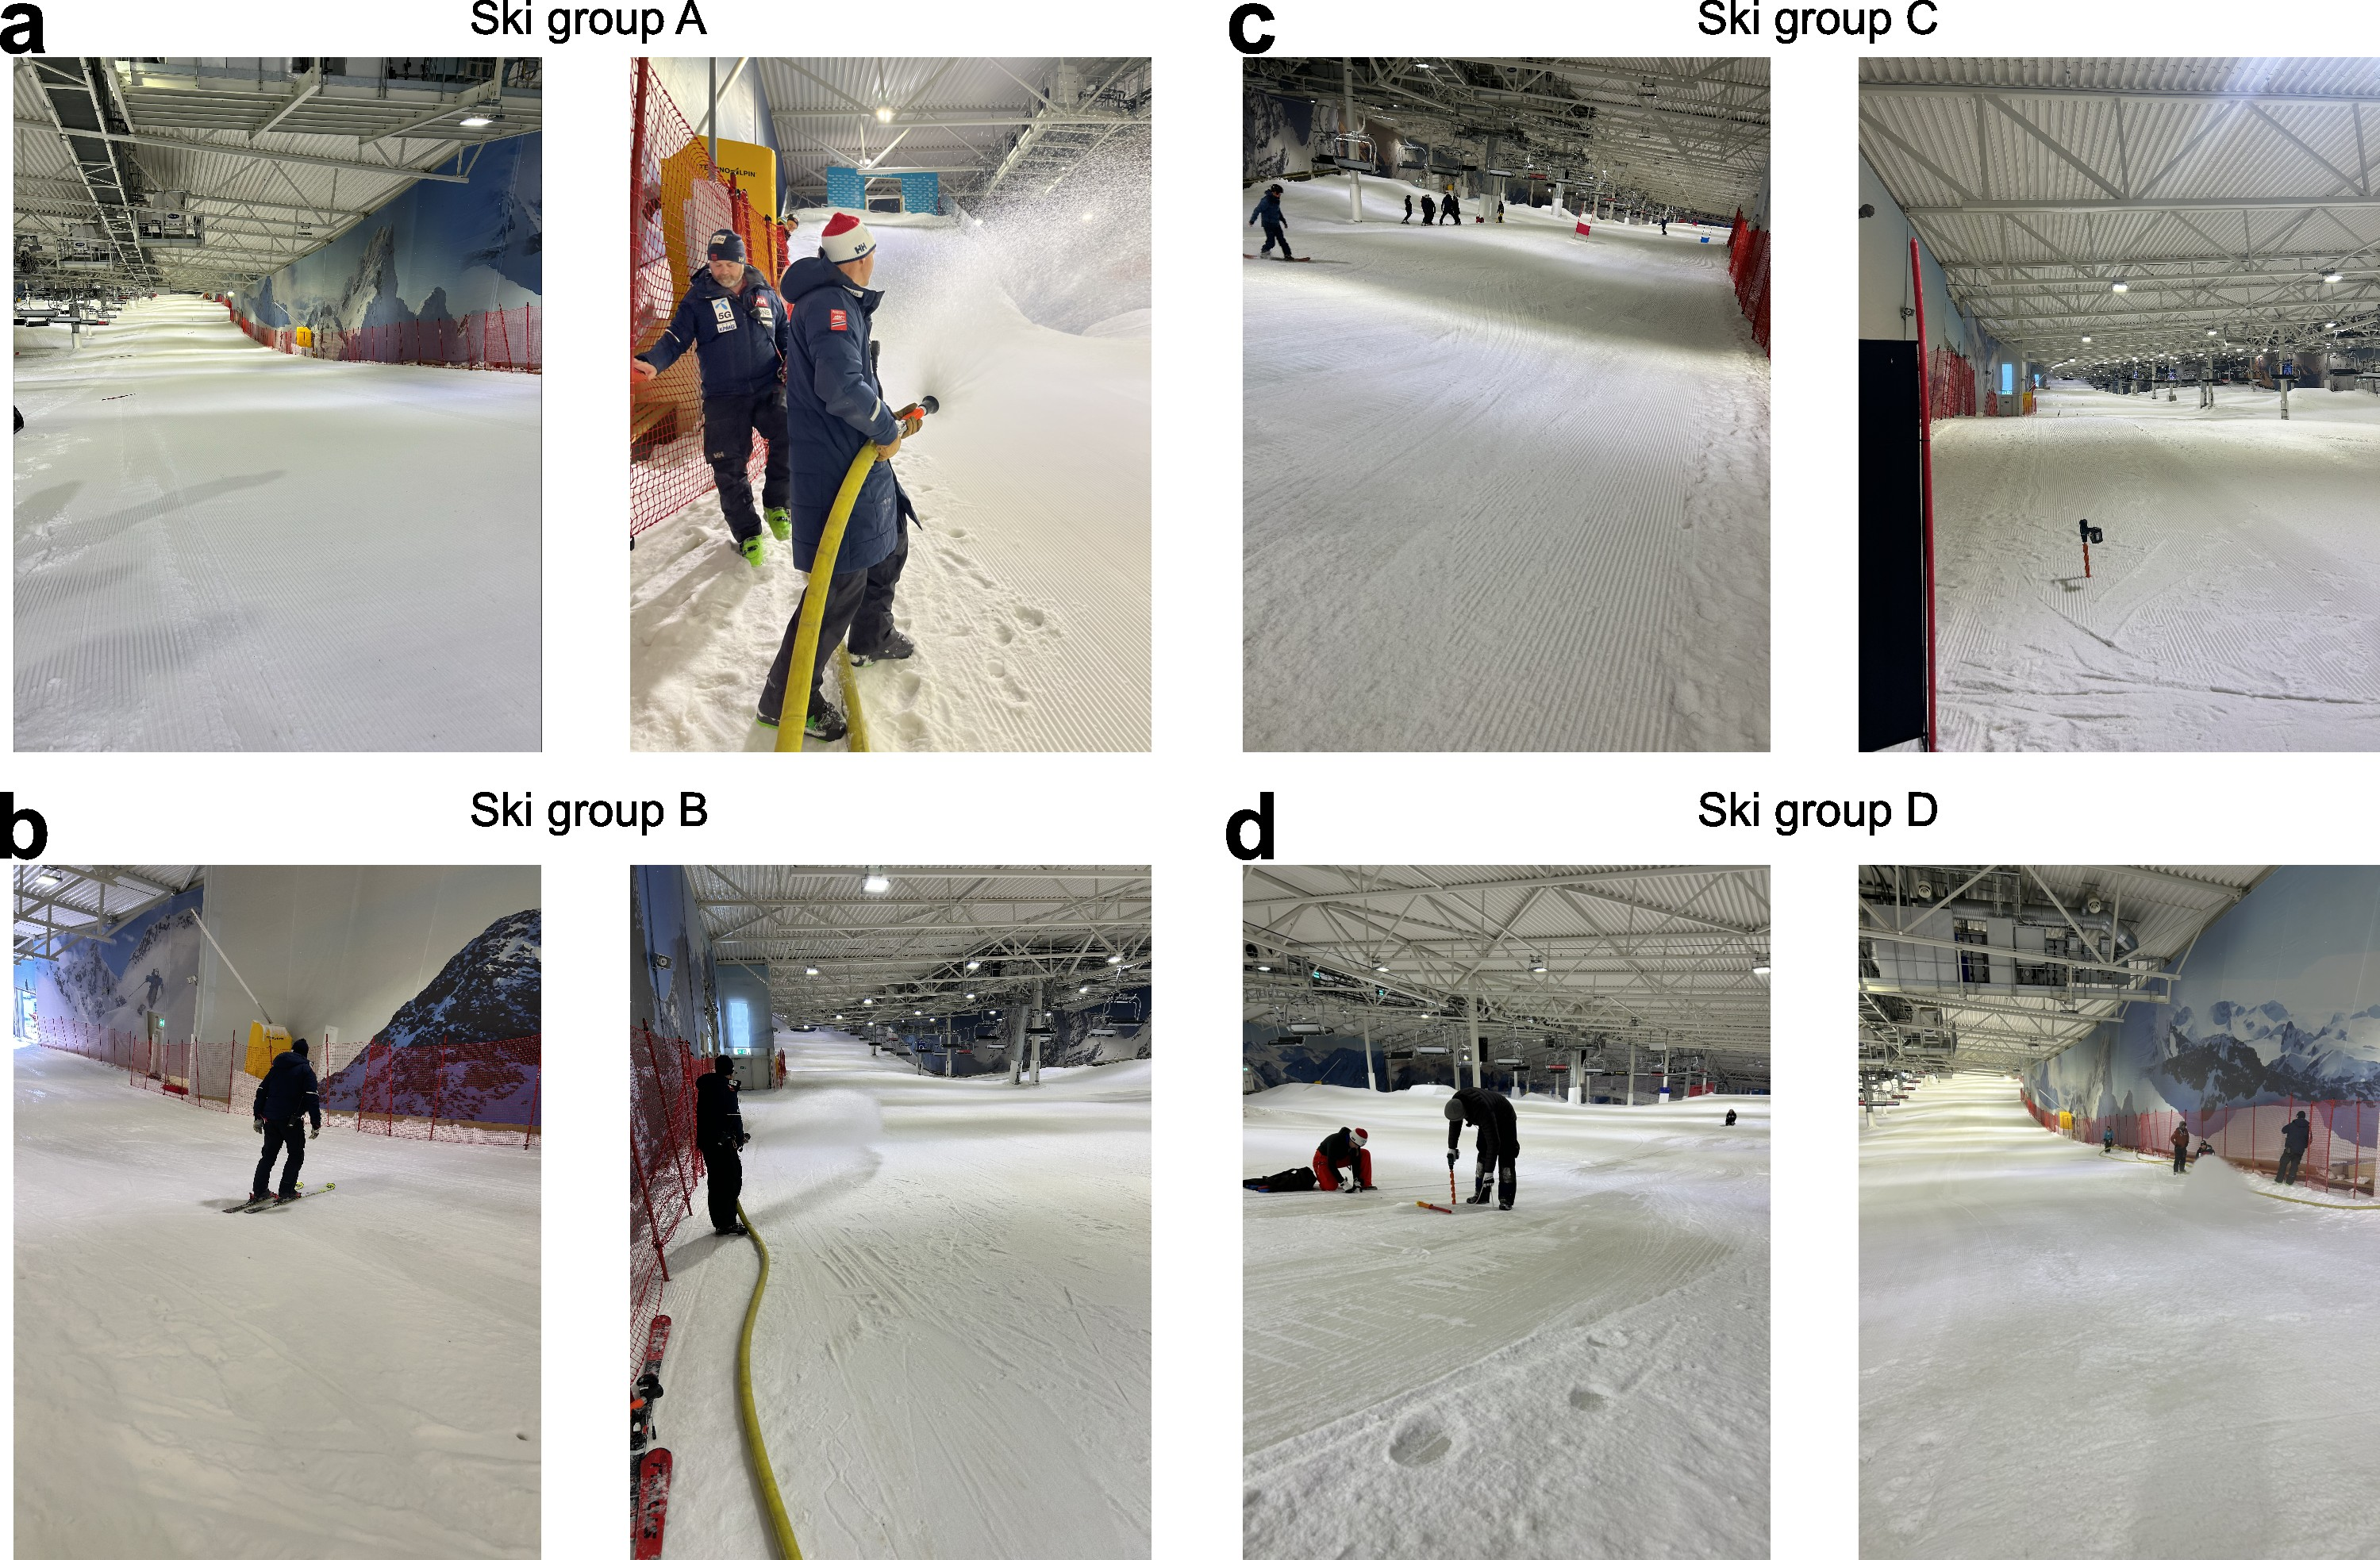
\includegraphics[width=\linewidth]{figures/figure_appendix_snowprep.jpg}
\caption{Images showing the hill preparation for the four ski groups. \textbf{a}. Shows the racing hill for ski group A. The left image displays the racing hill the evening before data collection after it was groomed. The right image shows the watering process for ski group A. \textbf{b}. Shows the racing hill for ski group B. The left image depicts the course inspection immediately after ski group A finished their testing. The right image shows the watering process for ski group B. Note that we did not groom the course this time, so in the image, you can see some uneven surfaces on the snow, which were evened out by watering it. \textbf{c}. Shows the racing hill for ski group C. The left image displays the hill after it was groomed and left overnight. The right image shows the same but from the bottom. \textbf{d}. Shows the racing hill for ski group D. The left image illustrates the hill for ski group C on their retention test. Note the icy surface, which was the reason why we produced new snow. The right image shows the watering process for ski group D. 
}
\label{fig:snowprep}
\end{figure}
 
\subsubsection*{Ski group D}
After Ski Group C, the race hill needed new snow because some areas had become icy, with minimal grip (Fig. ref{fig:snowprep}d:left)). Although the conditions were suitable for Ski Group C, they would not have worked for a new ski group undergoing testing. Consequently, we decided to produce new snow two days before Ski Group D started their training. This fresh snow was pushed into the racing hill the day before testing and groomed. Subsequently, we watered the hill and let it freeze overnight (Fig. \ref{fig:snowprep}d:right)


\subsection{Course setting}\label{secA2}
We used a standard procedure to set the slalom courses, ensuring a fixed length and offset. First, we stretched a taut rope between two nails on either side of the ski hill. This rope helped us locate the exact starting line consistently from day to day. From the nail on the skier's right, we measured 6 meters into the slope. We did the same from a fixed point approximately 50 meters down the course, but here we measured 3.4 meters out. Then, we pulled a 50-meter-long measuring tape between the two points to establish the line down the hill   We chose a measuring tape over a rope because ropes tend to expand and contract when they get wet and dry, respectively (see Fig.\ref{fig:coursesetting}a for an image illustrating this process).

\begin{figure}[h!]
\centering
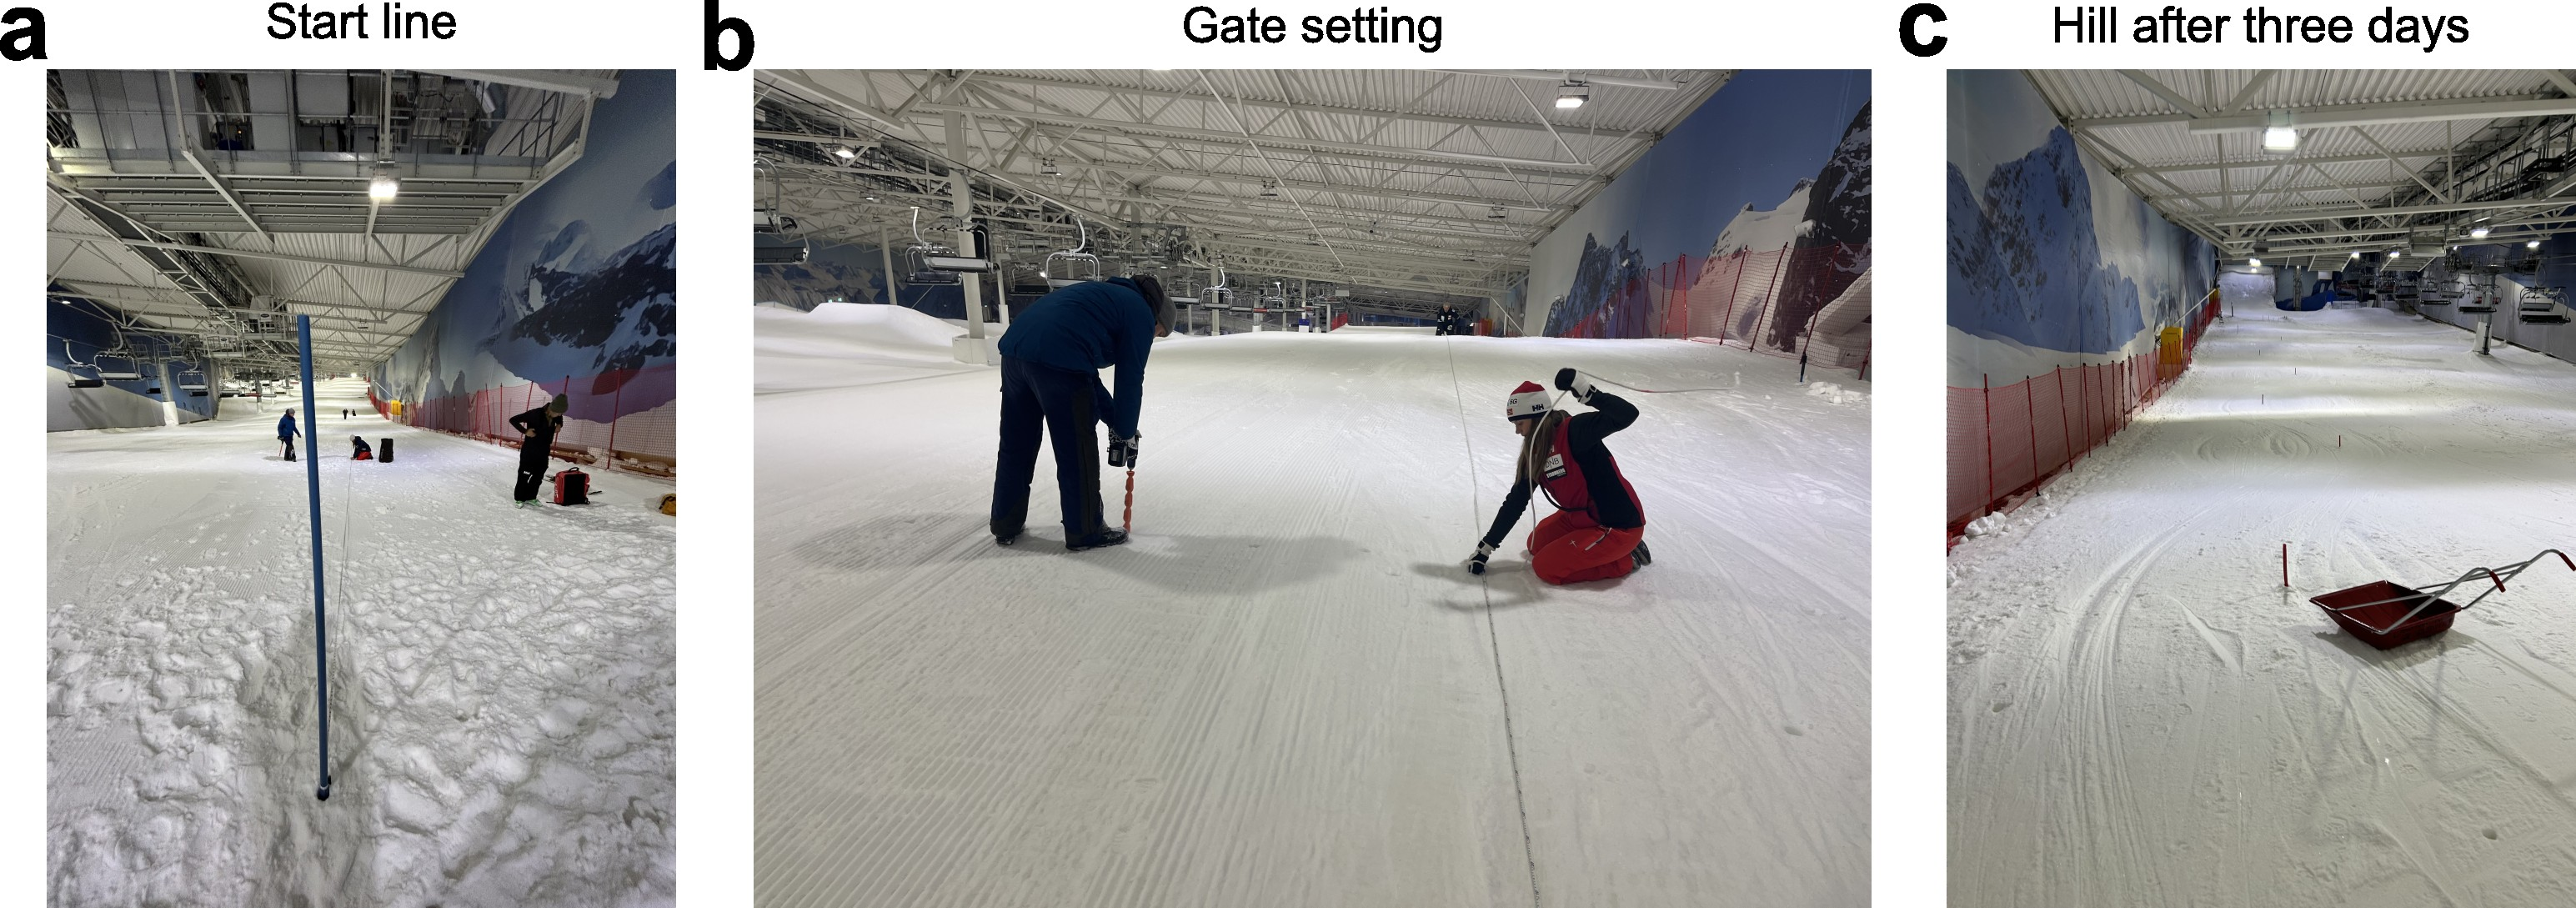
\includegraphics[width=\linewidth]{figures/figure_appendix_coursesetting.jpg}
\caption{Images showing the procedure for course setting. \textbf{a}. The image illustrates the process of establishing the straight reference line down the hill. The long blue gate is positioned 6 meters from the nail on the skier's right. \textbf{b}. This image showcases the gate-setting method. A white rope is secured to the reference line with a carabiner hook, and a marker on the rope indicates a distance of 1.9 meters for placing the gate. \textbf{c}. The image reveals the tracks left behind by a group of skiers that was tested
}
\label{fig:coursesetting}
\end{figure}
 

Once the 50-meter straight line was established, we laid out a rope segment attached to a carabiner hooked onto the long rope. We moved this segment 1.9 meters out from the rope in one turn and 0 meters in the other, with a 10-meter vertical space. This ensured that the course followed a straight line down the slope and was set with the correct offset (see figure\ref{fig:coursesetting}b for an image illustrating this process). Once all the gates along the 50-meter measurement tape were set, we used a new fixation point down the slope and continued down the course. We practiced this procedure several times before the experiment, and the variation in course setting was a maximum of 10 cm at the end of the course.

Due to wear and tear on the trails, we opted to shift the course laterally or rotate it, depending on the situation. With the exception of one skiing group, we followed the following practice. On day 1, we set the course as described above. On day 2, we rotated the course so that the first turn went in the opposite direction of day 1. On the third day, we shifted the course closer to the wall on skiers' right (see figure \ref{fig:coursesetting}c for an image showing the tracks in the hill left after a skigroup had completed the experiment). 












\end{document}
